\chapter{THEORETICAL BASIS}

\renewcommand{\headrulewidth}{0.5pt}
\renewcommand{\footrulewidth}{0.5pt}
\thispagestyle{plain}
\pagestyle{fancy}
\fancyhf{}
\fancyhead[L]{\textbf{CHAPTER 2}}
\fancyhead[R]{\textbf{DROWSINESS DETECTION AND ALERT SYSTEM IN THE CAR}}
\raggedright
\fancyfoot[L]{From: Nguyen Van Anh Tuan}
\fancyfoot[R]{Page \thepage}

\section{Overview About Image Processing}
    \subsection{Introduction about Image Processing}
        Image processing is a method to perform some operations on an image, 
        in order to get an enhanced image or to extract some useful information from it. It is a type of signal 
        processing in which input is an image and output may be image or characteristics/features associated with 
        that image. Nowadays, image processing is among rapidly growing technologies. It forms core research area 
        within engineering and computer science disciplines too. \\ 
        \vspace{3mm}
        Image processing basically includes the following 3 steps:
        \begin{itemize}
            \item Importing the image via image acquisition tools
            \item Analysing and manipulating the image
            \item Output in which result can be altered image or report that is based on image analysis
        \end{itemize}
        There are two types of methods used for image processing namely, analogue and digital image processing. 
        Analog image processing can be used for the hard copies like printouts and photographs. Image analysts use 
        various fundamentals of interpretation while using these visual techniques. Digital image processing techniques 
        help in manipulation of the digital images by using computers. The three general phases that all types of data 
        have to undergo while using digital technique are pre-processing, enhancement, and display, information extraction.
        \begin{figure}[H]
            \centering
            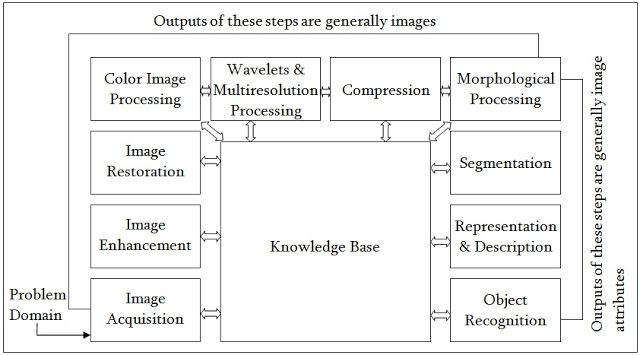
\includegraphics[width=0.6\linewidth]{img/IP.jpg}
            \caption{Fundamental steps in digital processing}
        \end{figure}
        \subsubsection{Image Acquistion}
            This is the first step or process of the fundamental steps of digital image processing. Image acquisition could 
            be as simple as being given an image that is already in digital form. Generally, the image acquisition stage involves 
            preprocessing, such as scaling etc.
        \subsubsection{Image Enhancement}
            Image enhancement is among the simplest and most appealing areas of digital image processing. Basically, the idea behind 
            enhancement techniques is to bring out detail that is obscured, or simply to highlight certain features of interest in an 
            image. Such as, changing brightness \& contrast etc.
        \subsubsection{Image Restoration}
            Image restoration is an area that also deals with improving the appearance of an image. However, unlike enhancement, 
            which is subjective, image restoration is objective, in the sense that restoration techniques tend to be based on mathematical 
            or probabilistic models of image degradation.
        \subsubsection{Color Image Processing}
            Color image processing is an area that has been gaining its importance because of the significant increase in the use of digital 
            images over the Internet. This may include color modeling and processing in a digital domain etc.
        \subsubsection{Wavelets and Multiresolution Processing}
            Wavelets are the foundation for representing images in various degrees of resolution. Images subdivision successively into smaller 
            regions for data compression and for pyramidal representation.
        \subsubsection{Compression}
            Compression deals with techniques for reducing the storage required to save an image or the bandwidth to transmit it. Particularly in 
            the uses of internet it is very much necessary to compress data.
        \subsubsection{Morphological Processing}
            Morphological processing deals with tools for extracting image components that are useful in the representation and description of shape.
        \subsubsection{Segmentation}
            Segmentation procedures partition an image into its constituent parts or objects. In general, autonomous segmentation is one of the most difficult 
            tasks in digital image processing. A rugged segmentation procedure brings the process a long way toward successful solution of imaging problems that 
            require objects to be identified individually.
        \subsubsection{Representation and Description}
            Representation and description almost always follow the output of a segmentation stage, which usually is raw pixel data, constituting either the boundary 
            of a region or all the points in the region itself. Choosing a representation is only part of the solution for transforming raw data into a form suitable 
            for subsequent computer processing. Description deals with extracting attributes that result in some quantitative information of interest or are basic for 
            differentiating one class of objects from another.
        \subsubsection{Object Recognition}
            Recognition is the process that assigns a label, such as, “vehicle” to an object based on its descriptors.
        \subsubsection{Knowledge Base}
            Knowledge may be as simple as detailing regions of an image where the information of interest is known to be located, thus limiting the search that has to be 
            conducted in seeking that information. The knowledge base also can be quite complex, such as an interrelated list of all major possible defects in a materials 
            inspection problem or an image database containing high-resolution satellite images of a region in connection with change-detection applications.
    \subsection{The Components of Image Processing}
        \subsubsection{Digital Image}
            A digital image is a finite set of pixels with a gray level suitable for describing an image close to the real image. The number of pixels 
            determines the resolution of the image. The higher quality of the image, the more clearly the image's points are displayed, making the image 
            more realistic and sharp.
        \subsubsection{Picture Element}
            In digital imaging, pixel, pel, or picture element is a smallest addressable element in a raster image, or the smallest addressable element in an \textbf{all points 
            addressable display device}; so it is the smallest controllable element of a picture represented on the screen. \\ 
            \vspace{3mm}
            Each pixel is a sample of an original image; more samples typically provide more accurate representations of the original. The intensity of each pixel is variable. 
            In color imaging systems, a color is typically represented by three or four component intensities such as red, green, and blue, or cyan, magenta, yellow, and black. \\ 
            \vspace{3mm}
            In some contexts (such as descriptions of \textbf{camera sensors}), pixel refers to a single scalar element of a multi-component representation (called a photosite in the 
            camera sensor context, although sensel is sometimes used), while in yet other contexts it may refer to the set of component intensities for a spatial position.
            \begin{figure}[H]
                \centering
                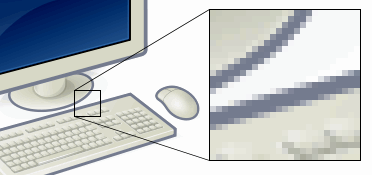
\includegraphics[width=0.6\linewidth]{img/Pixel-example.png}
                \caption{Pixel example}
            \end{figure}
            Pixel is an element of digital image at coordinate (x,y) with gray level or certain color. The size and the distance between those pixels are chosen appropriately so that 
            the human eye perceives spatial continuity and gray level (or color) of digital image like real image. Each of element in matrix is called an image element.
        \subsubsection{Gray Level of Picture}
            Gray level is the result of conversion of 1 luminosity value of 1 pixel positive integer value. Usually identified in [0,255] depending on the value each pixel is 
            represented. Common gray scale values is: 16, 32, 64, 128, 256 (level 256 is universal level). The reason is computer techniques use 1 byte (8 bits) to represent 
            the gray level. Gray level use 1 byte represent: 28 = level 256, it mean from 0 to 255).
            \begin{figure}[H]
                \centering
                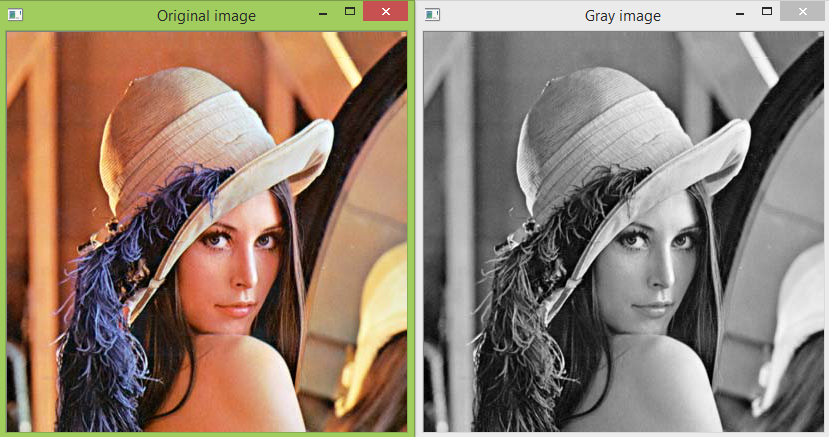
\includegraphics[width=0.6\linewidth]{img/gray-scale.png}
                \caption{Gray scale image example}
            \end{figure}
        \subsubsection{Image Resolution}
            Image resolution is detail an image holds. The term applies to raster digital images, film images, and other types of images. Higher resolution means more image detail. \\ 
            \vspace{3mm}
            Image resolution can be measured in various ways. Resolution quantifies how close lines can be to each other and still be visibly resolved. Resolution units can be tied 
            to physical sizes (e.g. lines per mm, lines per inch), to the overall size of a picture (lines per picture height, also knnown simply as lines, TV lines, or TVL), 
            or to angular subtense. Line pairs are often used instead of lines; a line pair comprises a dark line and an adjacent light line. A line is either a dark line or 
            a light line. A resolution of 10 lines per milimeter means 5 dark line alternating with 5 light lines, or 5 line pairs per milimeter (5 LP/mm). Photographic lens and film 
            resolution are most often quoted in line pairs per milimeter. \\ 
            \vspace{3mm}
            For example: Image resolution in CGA display (Color Graphic Adaptor) is a grid of points across the screen: 320 vertical points * 200 image points (320*200).
            Obviously, with the same CGA display 12 inches we notice smoother than the screen CGA 17 inches with resolution is 320*200. The reason is with the same resolution but 
            the larger the screen area, the less smooth.
        \subsubsection{Types of image classification}
            \begin{itemize}
                \item \textbf{Binary Image:} is one that consists of pixels that can have one of exactly two colors, usually black and white. Binary images are also called bi-level 
                or two-level, Pixelart made of two colours is often referred to as 1-Bit or 1bit. This means that each pixel is stored as a single bit—i.e., a 0 or 1. \\
                \vspace{2mm}
                The names black-and-white, B\&W, monochrome or monochromatic are often used for this concept, but may also designate any images that have only one sample per pixel, 
                such as grayscale images. In Photoshop parlance, a binary image is the same as an image in "Bitmap" mode. \\ 
                \vspace{2mm}
                Binary images often arise in digital image processing as masks or thresholding, and dithering. Some input/output devices, such as laser printers, fax machines, 
                and bilevel computer displays, can only handle bilevel images. \\ 
                \vspace{2mm}
                A binary image can be stored in memory as a bitmap, a packed array of bits. A 640×480 image requires 37.5 KiB of storage. Because of the small size of the image files, 
                fax machine and document management solutions usually use this format. Most binary images also compress well with simple run-length compression schemes. \\ 
                \vspace{2mm}
                Binary images can be interpreted as subsets of the two-dimensional integer lattice $Z^2$; the field of morphological image processing was largely inspired by this view.
                \item \textbf{RGB Image:} RGB Color Model is an additive color model, in which red, green, and blue light are added together in various ways to reproduce a broad array 
                of colors. The name of the model comes from the initials of the three additive primary colors, red, green, and blue. \\ 
                \vspace{2mm}
                RGB is a device-dependent color model: different devices detect or reproduce a given RGB value differently, since the color elements (such as phosphors or dyes) 
                and their response to the individual R, G, and B levels vary from manufacturer to manufacturer, or even in the same device over time. Thus an RGB value does not define 
                the same color across devices without some kind of color management.
                \begin{figure}[H]
                    \centering
                    
\includegraphics[width=0.6\linewidth]{img/RGB.png}
                    \caption{Additive color mixing}
                \end{figure}
                The choice of primary colors is related to the physiology of the human eye; good primaries are stimuli that maximize the difference between the responses of the cone 
                cells of the human retina to light of different wavelengths, and that thereby make a large color triangle. \\ 
                \vspace{2mm}
                The normal three kinds of light-sensitive photoreceptor cells in the human eye (cone cells) respond most to yellow (long wavelength or L), green (medium or M), 
                and violet (short or S) light (peak wavelengths near 570 nm, 540 nm and 440 nm, respectively). The difference in the signals received from the three kinds allows 
                the brain to differentiate a wide gamut of different colors, while being most sensitive (overall) to yellowish-green light and to differences between hues in the 
                green-to-orange region.
                \begin{figure}[H]
                    \centering
                    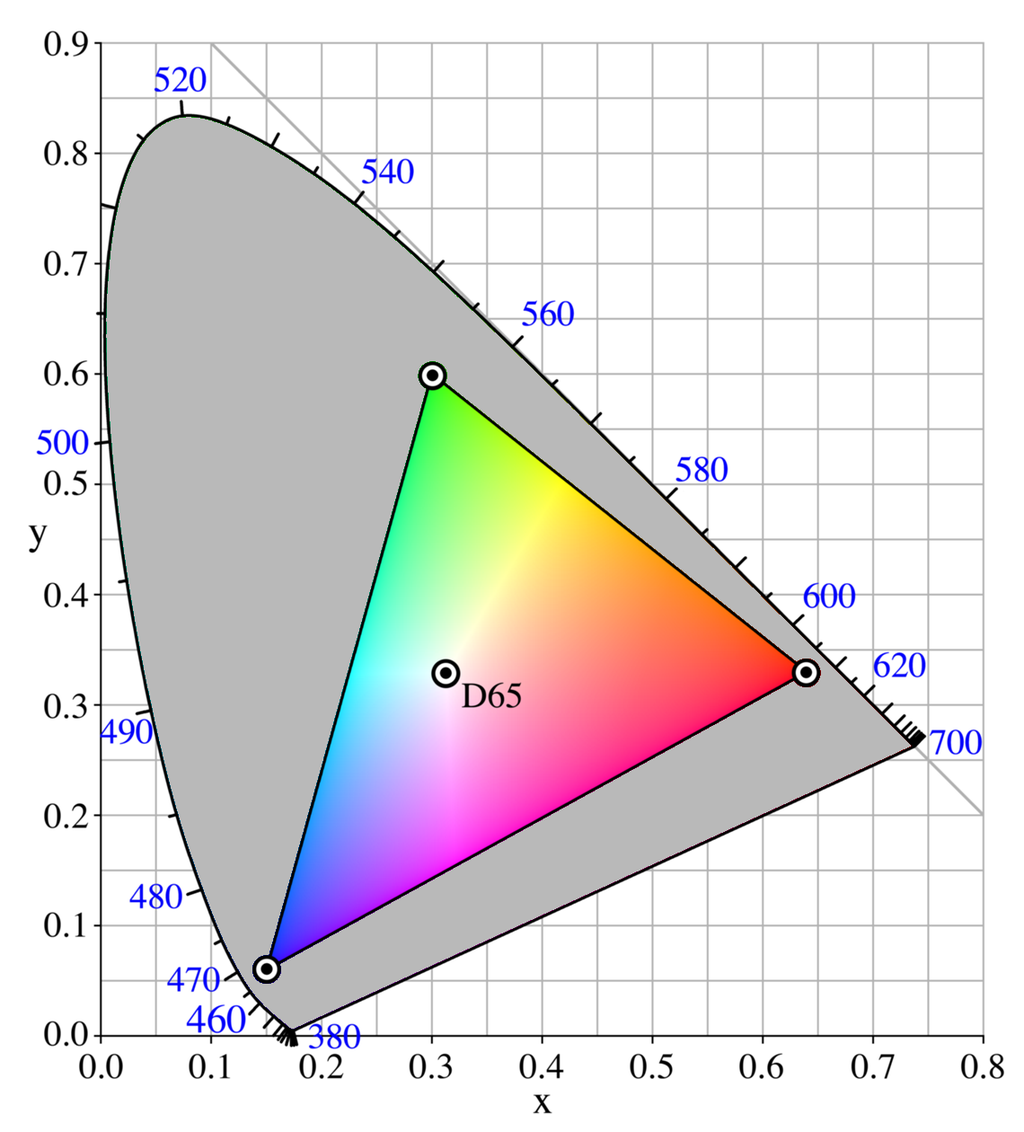
\includegraphics[width=0.6\linewidth]{img/primary-color.png}
                    \caption{A set of primary colors, such as the sRGB primaries, define a color triangle}
                \end{figure}
                \item \textbf{Image Transformation:} is a function. A function that maps one set to another set after performing some operations. \\ 
                \vspace{2mm}
                Image transformation is consider this equation:
                \begin{align}
                    G(x,y) = T{f(x,y)}
                \end{align}
                In this equation, $F(x,y)$ is input image on which transformation function has to be applied; $G(x,y)$ is the output image or processed image; $T$ is the transformation 
                function. This relation between input image and the processed output image can also be represented as: $s = T(r)$ where $r$ is actually the pixel value or gray level intensity 
                of $f(x,y)$ at any point. And $s$ is the pixel value or gray level intensity of $g(x,y)$ at any point. \\
                \vspace{2mm}
                The basic gray level transformation has been discussed in our tutorial of basic gray level transformations. There is some image transformations like: \texttt{Fourier Transform, Cousin, 
                Sin, convolution transform, Kronecker product}.
            \end{itemize}
    \subsection{Parts of The Image Processing System}
        \begin{figure}[H]
            \centering
            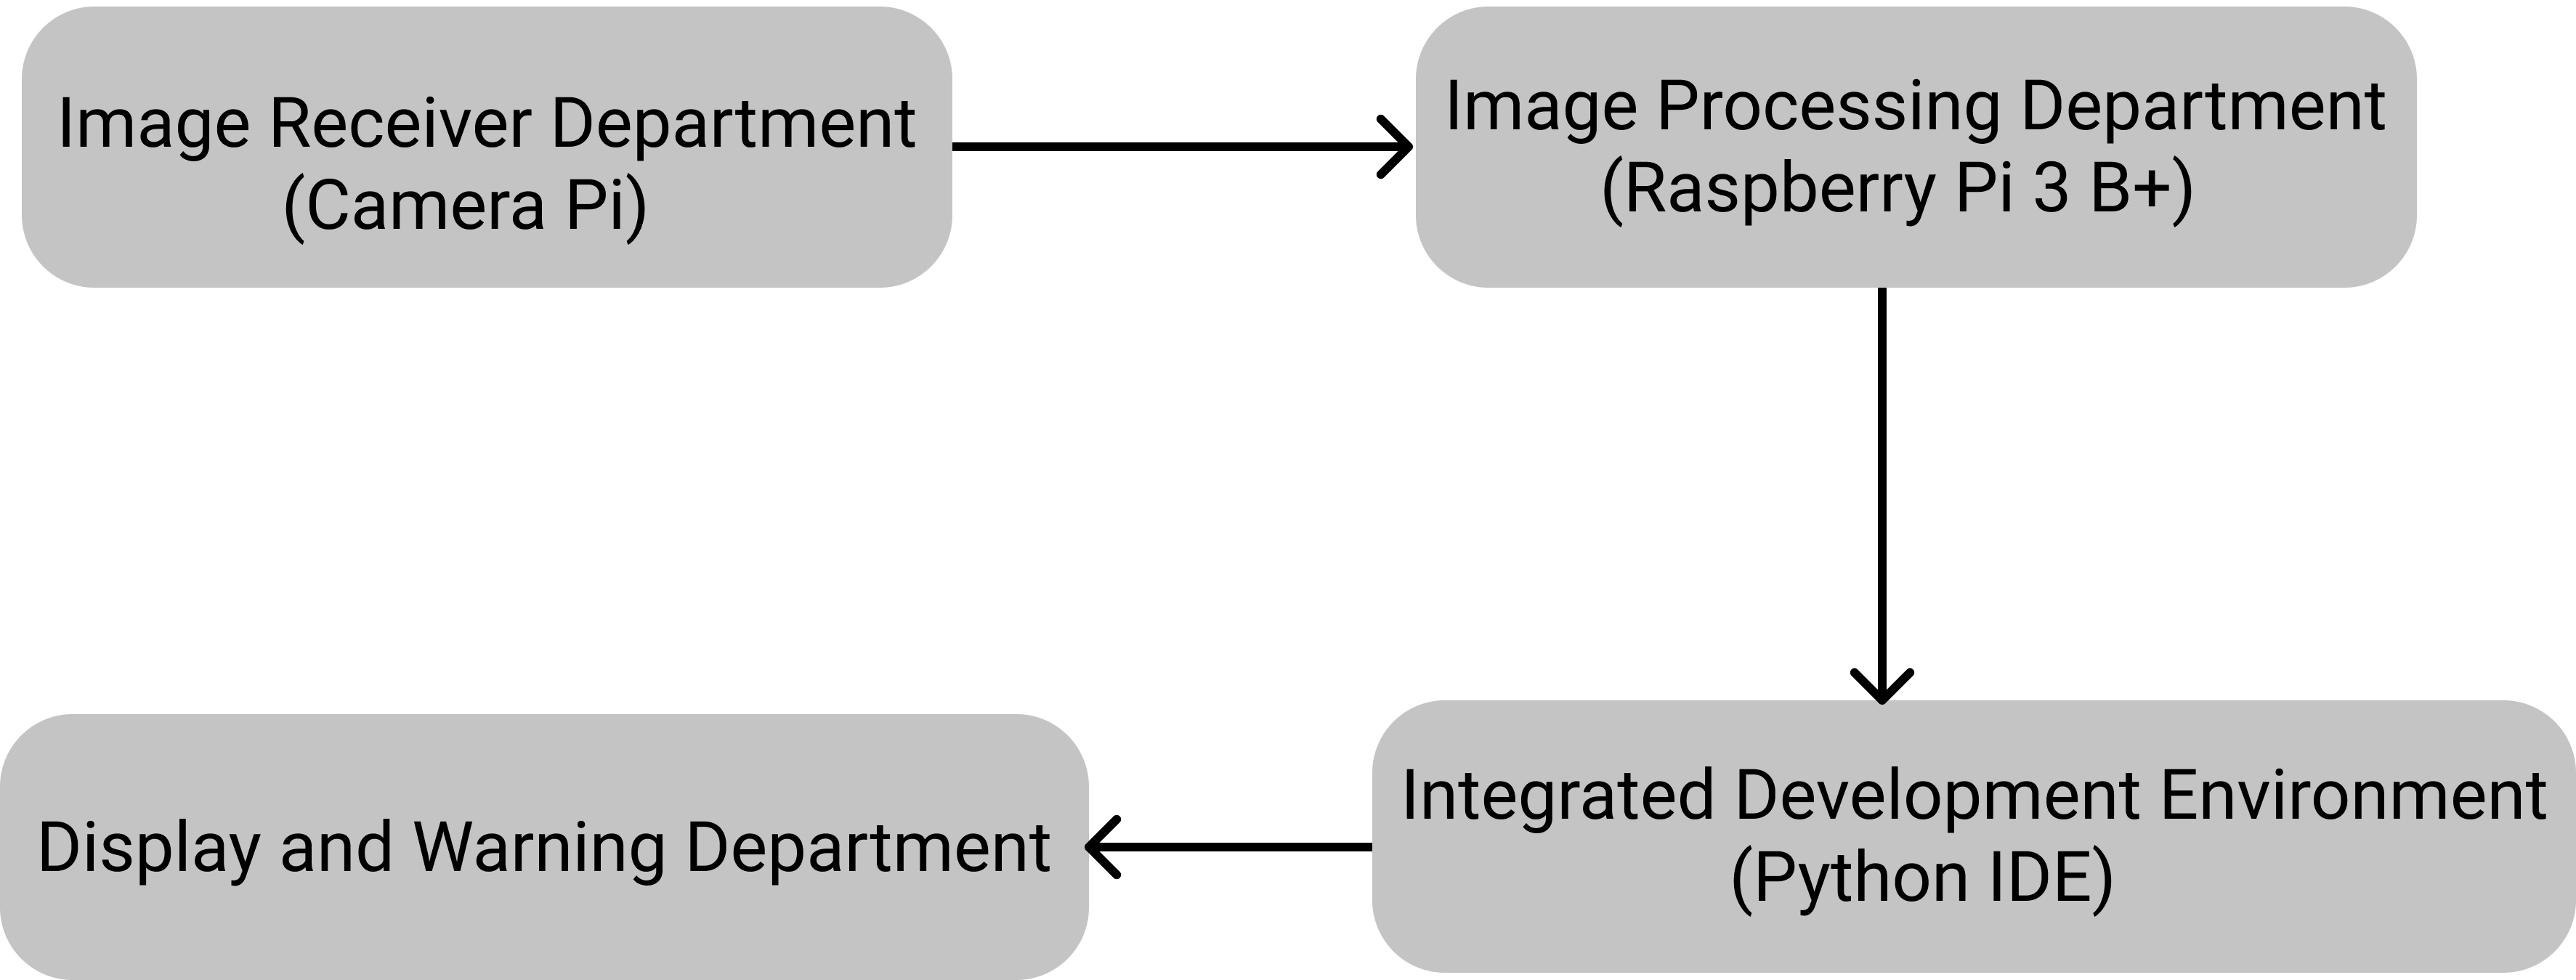
\includegraphics[width=0.6\linewidth]{img/Drowsiness.png}
            \caption{The part of image processing system}
        \end{figure}
        \textbf{Image Receiver Department} is usually a camera, scaners, image sensor,... In this project, a pi camera with 5mpx resolution is used to capture images. \\ 
        \vspace{3mm}
        \textbf{Image Processing Department} is specialized processing equipment or computers,... Specifically here using a Raspberry pi 3B + computer for image processing. \\ 
        \vspace{3mm}
        \textbf{Integrated Development Environment} using Thony Python IDE software to write program. \\ 
        \vspace{3mm}
        \textbf{Warning Devices} speaker alarms.

\section{Face Regconition Algorithm}
    Before we go to the algorithms for face detection we should understand how to detect a face even though we don't know who the subject is. \\
    \vspace{3mm}
    Face Recognition is a way of recognizing a human face through technology. A facial recognition system uses biometrics to map facial features from a photograph or video. 
    It compares the information with a database of known faces to find a match. Facial recognition can help verify personal identity, but it also raises privacy issues. \\ 
    \vspace{3mm}
    The recognition of a face in a video sequence is split into three primary tasks: Face Detection, Face Prediction, and Face Tracking. The tasks performed in the Face Capture 
    program are performed during face recognition as well. To recognize the face obtained, a vector of HOG features of the face is extracted. This vector is then used in the SVM 
    model to determine a matching score for the input vector with each of the labels. The SVM returns the label with the maximum score, which represents the confidence to the 
    closest match within the trained face data. 
    \begin{figure}[H]
        \centering
        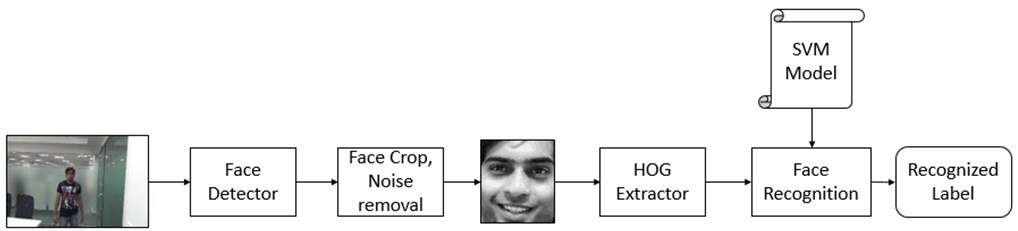
\includegraphics[width=0.6\linewidth]{img/face-recognition.jpg}
        \caption{Block diagram of the face recognition process}
    \end{figure}
    The task of calculating matching scores is exceptionally heavy to compute. Hence, once detected and identified, the labeled face in an image needs to be tracked to reduce the 
    computation in future frames until the face eventually disappears from the video. Of all the available trackers, the Camshift tracking algorithm is used since it produces the 
    best results with faces. \\ 
    \vspace{3mm}
    Where you see a face, recognition technology sees data. That data can be stored and accessed. 
    For instance, half of all American adults have their images stored in one or more facial-recognition databases that law enforcement agencies can search, according to a 
    Georgetown University study. Technologies can be different, but there are the basic steps:
    \begin{itemize}
        \item \textbf{Step 1.} A picture of your face is captured from a photo or video. Your face might appear alone or in a crowd. Your image may show you looking straight 
        ahead or nearly in profile
        \item \textbf{Step 2.} Facial recognition software reads the geometry of your face. Key factors include the distance between your eyes and the distance from forehead to chin. 
        The software identifies facial landmarks — one system identifies 68 of them — that are key to distinguishing your face. The result: your facial signature
        \item \textbf{Step 3.} Your facial signature — a mathematical formula — is compared to a database of known faces. And consider this: at least 117 million Americans have images 
        of their faces in one or more police databases. According to a May 2018 report, the FBI has had access to 412 million facial images for searches
        \item \textbf{Step 4.} A determination is made. Your faceprint may match that of an image in a facial recognition system database.
    \end{itemize}
    The gist of the pipeline can be seen in figure down here: 
    \begin{figure}[H]
        \centering
        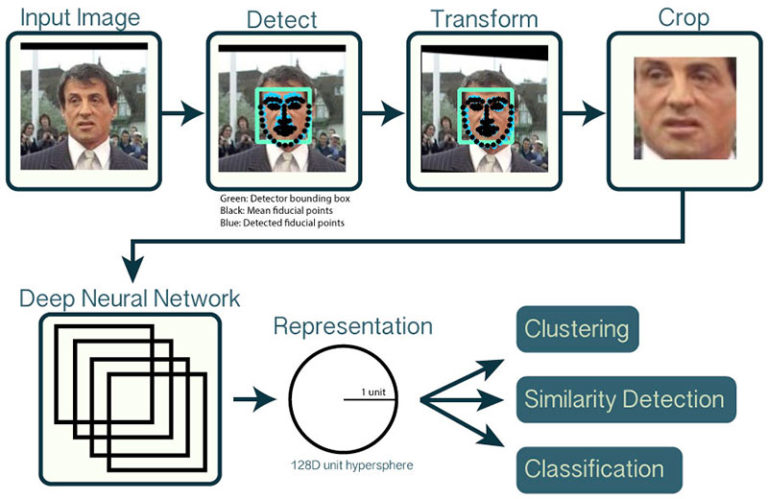
\includegraphics[width=0.6\linewidth]{img/opencv.jpg}
        \caption{An overview of the OpenCV face recognition pipeline}
    \end{figure}
    First, we input an image or video frame to our face recognition pipeline. Given the input image, we apply face detection to detect the location of a face in the image. Optionally 
    we can compute \textbf{Facial Landmarks}, enabling us to \textbf{Preprocess and align the face}. \\ 
    \vspace{3mm}
    Face alignment, as the name suggests, is the process of identifying the geometric structure of the faces and attempting to obtain a canonical alignment of the face based on translation, 
    rotation, and scale. While optional, face alignment has been demonstrated to increase face recognition accuracy in some pipelines. After we’ve (optionally) applied face alignment 
    and cropping, we pass the input face through our deep neural network:
    \begin{figure}[H]
        \centering
        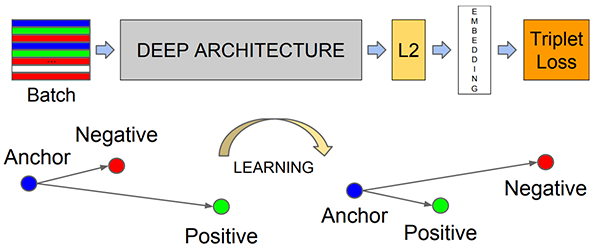
\includegraphics[width=0.6\linewidth]{img/pyimgsearch.png}
        \caption{How the deep learning face recognition model computes the face embedding}
    \end{figure}
    The FaceNet deep learning model computes a 128-d embedding that quantifies the face itself. But how does the network actually compute the face embedding? The answer lies in the training 
    process itself, including:
    \begin{itemize}
        \item The input data to the network
        \item The triplet loss function
    \end{itemize}
    To train a face recognition model with deep learning, each input batch of data includes three images:
    \begin{itemize}
        \item The anchor
        \item The positive image
        \item The negative image
    \end{itemize}
    The anchor is our current face and has identity A. \\ 
    \vspace{3mm}
    The second image is our positive image — this image also contains a face of person A. \\ 
    \vspace{3mm}
    The negative image, on the other hand, does not have the same identity, and could belong to person B, C, or even Y! \\
    \vspace{3mm}
    The point is that the anchor and positive image both belong to the same person/face while the negative image does not contain the same face. The neural network computes the 128-d 
    embeddings for each face and then tweaks the weights of the network (via the triplet loss function) such that:
    \begin{itemize}
        \item The 128-d embeddings of the anchor and positive image lie closer together
        \item While at the same time, pushing the embeddings for the negative image father away
    \end{itemize}
    In this manner, the network is able to learn to quantify faces and return highly robust and discriminating embeddings suitable for face recognition.
    \subsection{Face Detection using HOG}
        The essential thought behind the histogram of oriented gradients descriptor is that local object appearance and shape within an image can be described by the distribution of intensity gradients or edge directions. 
        The image is divided into small connected regions called cells, and for the pixels within each cell, a histogram of gradient directions is compiled. The descriptor is the concatenation of these histograms. For 
        improved accuracy, the local histograms can be contrast-normalized by calculating a measure of the intensity across a larger region of the image, called a block, and then using this value to normalize all cells 
        within the block. This normalization results in better invariance to changes in illumination and shadowing. \\
        \vspace{3mm}
        In the current example, all the face sample images of a person are fed to the feature descriptor extraction algorithm; i.e., a HOG. The descriptors are gradient vectors generated per pixel of the image. 
        The gradient for each pixel consists of magnitude and direction, calculated using the following formular:
        \begin{figure}[H]
            \centering
            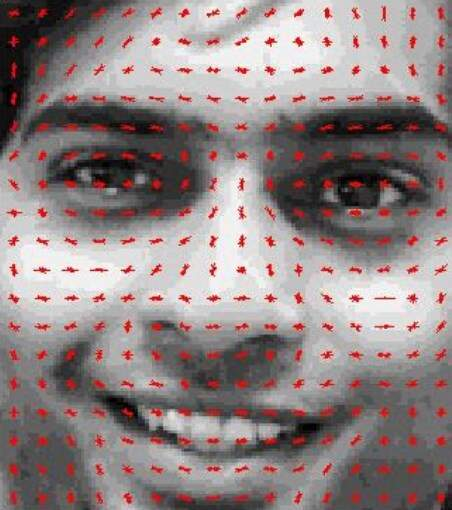
\includegraphics[width=0.6\linewidth]{img/HOG-feature.jpg}
            \caption{HOG features sample face}
        \end{figure}
        \begin{align}
            g = \sqrt{g^2_x + g^2_y} \\ 
            \theta = \arctan{\frac{g_y}{g_x}}
        \end{align}
        Gx and Gy are respectively the horizontal and vertical components of the change in the pixel intensity. A window size of 128 x 144 is used for face images since it matches the general aspect ratio of human faces. 
        The descriptors are calculated over blocks of pixels with 8 x 8 dimensions. These descriptor values for each pixel over 8 x 8 block are quantized into 9 bins, where each bin represents a directional angle of gradient 
        and value in that bin, which is the summation of the magnitudes of all pixels with the same angle. \\ 
        \vspace{3mm}
        Further, the histogram is then normalized over a 16 x 16 block size, which means four blocks of 8 x 8 are normalized together to minimize light conditions. This mechanism mitigates the accuracy drop due to a 
        change in light. The SVM model is trained using a number of HOG vectors for multiple faces. \\
        \vspace{3mm}
        There is some review entire detailed process of training an object detector using Histogram Oriented Gradients, each step can be fairly detailed. It goes like something like this:
        \begin{itemize}
            \item \textbf{Step 1:} Sample P positive samples from your training data of the object(s) you want to detect and extract HOG descriptors from these samples;
            \item \textbf{Step 2:} Sample N negative samples from a negative training set that \textbf{does not contain} any of the objects you want to detect and extract HOG descriptors from these samples as well. In practice N $\gg$ P;
            \item \textbf{Step 3:} Train a Linear Support Vector Machine on your positive and negative samples;
            \item \textbf{Step 4:} 
                \begin{figure}[H]
                    \centering
                    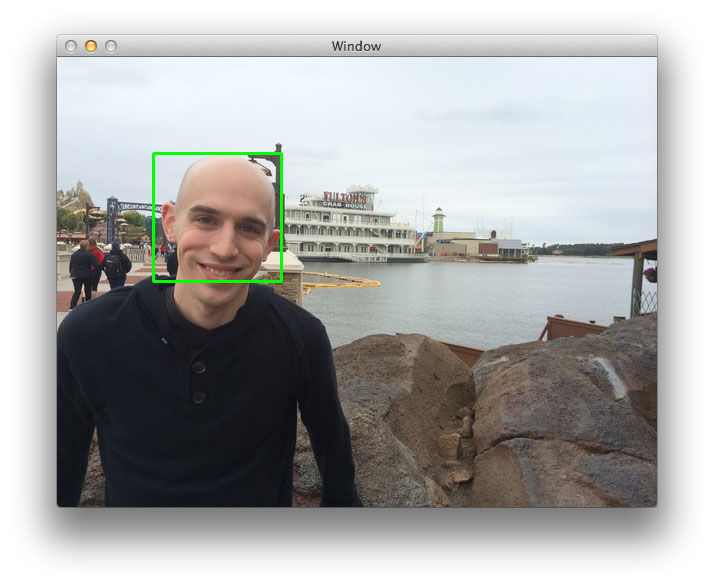
\includegraphics[width=0.6\linewidth]{img/sliding_window_example.jpg}
                    \caption{Example of the sliding a window approach, where we slide a window from left-to-right and top-to-bottom}
                \end{figure}
                \textbf{Apply hard-negative mining}, For each image and each possible scale of each image in your negative training set, apply the sliding window technique and slide your window across the image. 
                At each window compute your HOG descriptors and apply your classifier. If your classifier (incorrectly) classifies a given window as an object (and it will, there will absolutely be false-positives), 
                record the feature vector associated with the false-positive patch along with the probability of the classification. \textbf{This approach is called hard-negative mining}.
            \item \textbf{Step 5:} Take the false-positive samples found during the hard-negative mining stage, sort them by their confidence (i.e. probability) and re-train your classifier using these hard-negative samples.
            \item \textbf{Step 6:} Your classifier is now trained and can be applied to your test dataset. Again, just like in Step 4, for each image in your test set, and for each scale of the image, apply the sliding window technique. 
                At each window extract HOG descriptors and apply your classifier. If your classifier detects an object with sufficiently large probability, record the bounding box of the window. After you have finished scanning the image, 
                apply non-maximum suppression to remove redundant and overlapping bounding boxes. \\ 
                \vspace{2mm}
                These are the bare minimum steps required, but by using this 6-step process you can train and build object detection classifiers of your own! Extensions to this approach include a deformable parts model and Exemplar SVMs, 
                where you train a classifier for each positive instance rather than a collection of them. \\ 
                \vspace{2mm}
                However, if you’ve ever worked with object detection in images you’ve likely ran into the problem of detecting multiple bounding boxes around the object you want to detect in the image. And here’s an example of this overlapping bounding box problem:
                \begin{figure}[H]
                    \centering
                    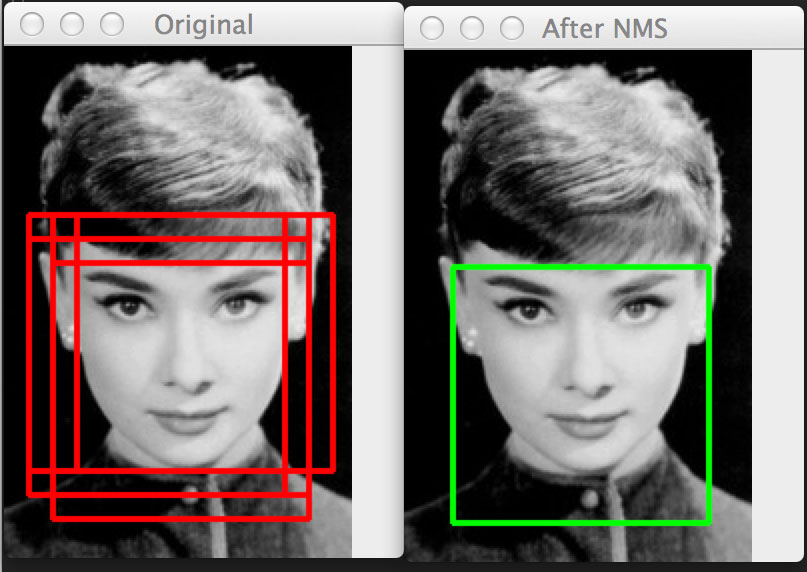
\includegraphics[width=0.6\linewidth]{img/multiple-overlapping.jpg}
                    \caption{(Left) Detecting multiple overlapping bounding boxes around the face we want to detect. (Right) Applying non-maximum suppression to remove the redundant bounding boxes.}
                \end{figure}
        \end{itemize}
    \subsection{Haar-like Feature (Haar-Cascade)}
        \subsubsection{Theory}
            Object Detection using Haar feature-based cascade classifiers is an effective object detection method is a machine learning based approach where a cascade function is trained from a lot of positive and negative images. It is then used to detect objects in other images. \\ 
            \vspace{3mm}
            Here we will work with face detection. Initially, the algorithm needs a lot of positive images (images of faces) and negative images (images without faces) to train the classifier. Then we need to extract features from it. For this, Haar features shown in the below image 
            are used. They are just like our convolutional kernel. Each feature is a single value obtained by subtracting sum of pixels under the white rectangle from sum of pixels under the black rectangle.
            \begin{figure}[H]
                \centering
                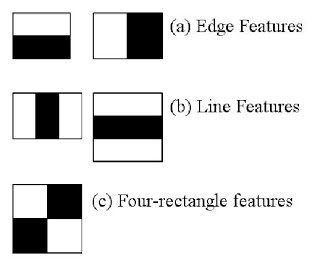
\includegraphics[width=0.6\linewidth]{img/haar_features.jpg}
                \caption{Feature 4 rectangle}
            \end{figure}
            \begin{figure}[H]
                \centering
                
\includegraphics[width=0.6\linewidth]{img/feature_center.png}
                \caption{Feature in center}
            \end{figure}
            Using above features, we can calculate the value of the Haar-Like feature as the difference between the sum of the pixels of the black area and the white area as shown in the following formula:
            \begin{align}
                F(x) = Sum of black area - Sum of white area (gray level of pixel)
            \end{align} 
            There is a concept called \textbf{"Integral Image"}, is the 2D array with the size equal to the size of the image to be Haar-Like feature, with each element of this array is computed by summing the pixels above and left of it.
        \subsubsection{Integral Image}
            The idea of this concept is transforming an input images into a summed-area table, where the value at any point (x, y) in that table is the sum of all the pixels above and to the left of (x, y), inclusive:
            \begin{align}
                P(x,y) = \Sigma_{x' \leq x, y' \leq y} i(x',y')
            \end{align}
            Where I(x,y) is the value of the integral image pixel in the position (x,y), while i(x,y) is the corresponding intensity in the original image. It is a recursive formula, hence, if we start from one corner of the input image, we will have the same result in the integral image. 
            To make it clearer, let’s see an example:
            \begin{figure}[H]
                \centering
                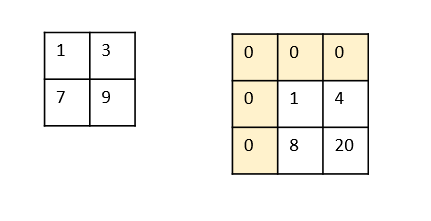
\includegraphics[width=0.6\linewidth]{img/example_integral.png}
                \caption{Example of Integral Image}
            \end{figure}
            In this figure we added one row and column of zeros, since we need one step backward in order to start the recursive formula. Hence, if your image is $w$ pixels wide and $h$ pixels high, then the integral of this will be $w+1$ pixels wide and $h+1$ pixels high. \\ 
            \vspace{3mm}
            Moving to the computations, let's start from the first pixel in the original image with intensity 1: the integral image returns exactly the same value, since it is computing (1+0+0). Then, pixel '3' becomes '4', since it is 3+1+0+0. With the same procedure, we obtain an 
            "8" (7+1+0) and a '20' (9+3+1+7). \\ 
            \vspace{3mm}
            We have a new image, but how is supposed to be useful? The answer rely in an unique property of the integral image. Indeed, it turned our that if you need to compute the summation within a window in the input image, hence that summation is equal to a linear combination 
            of the corresponding window’s corner in the integral image, as follows:
            \begin{align}
                \Sigma_{x_0 < x < x_1; y_0 < y < y_1} i(x,y) = I(D) + I(A) - I(B) - I(C)
            \end{align}
            Where is $A,B,C$ and $D$ are the corners of the corresponding window in the integral image.
            \begin{figure}[H]
                \centering
                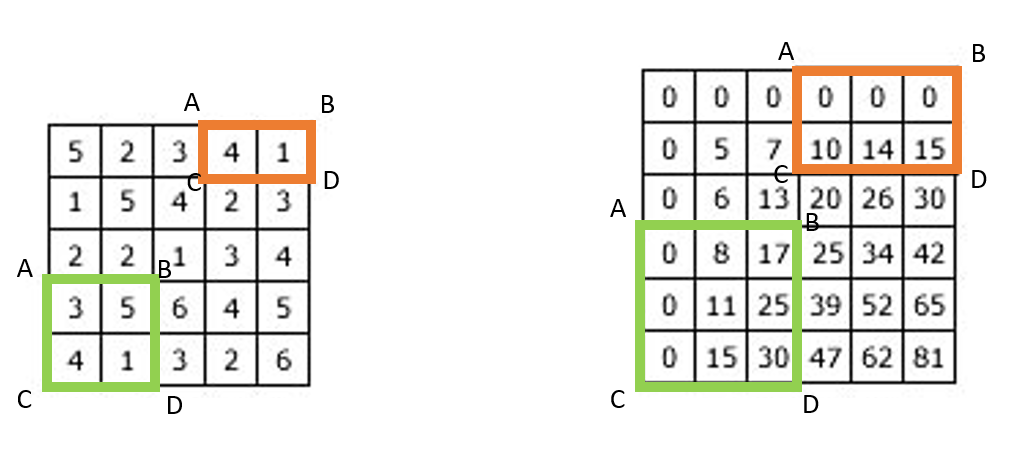
\includegraphics[width=0.6\linewidth]{img/corners_corresponding.png}
                \caption{Integral Image Approach}
            \end{figure}
            This reduces the number of computations by far. To give you an idea, consider a 100×100 image with a 9×9 window. We want to compute the sum of the pixel intensities within that window, which requires 8 operations. If we repeat this procedure 100 times, we obtain 800 operations. \\
            \vspace{3mm}
            Now let’s see the integral image approach. First, we compute the summed-area table, which requires 56 operations. Then, considering the same 9×9 window, to compute the sum of pixel intensity we just need the above formula, which is made of 3 operations. Hence, the total number 
            of operations is 56+3*100=356. As you can see, it is less than a half. \\
            \vspace{3mm}
            This procedure is widely used in computer vision and Haar Cascade algorithm is based exactly on that. \\
            \vspace{3mm}
            Now, all possible sizes and locations of each kernel are used to calculate lots of features. (Just imagine how much computation it needs? Even a 24x24 window results over 160000 features). For each feature calculation, we need to find the sum of the pixels under white 
            and black rectangles. To solve this, they introduced the integral image. However large your image, it reduces the calculations for a given pixel to an operation involving just four pixels. It makes things super-fast. \\ 
            \vspace{3mm}
            But among all these features we calculated, most of them are irrelevant. For example, consider the image below. The top row shows two good features. The first feature selected seems to focus on the property that the region of the eyes is often darker than the region of 
            the nose and cheeks. The second feature selected relies on the property that the eyes are darker than the bridge of the nose. But the same windows applied to cheeks or any other place is irrelevant. So how do we select the best features out of 160000+ features? 
            It is achieved by \textbf{Adaboost}.
            \begin{figure}[H]
                \centering
                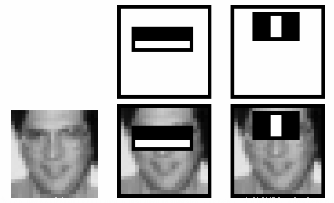
\includegraphics[width=0.6\linewidth]{img/haar_example.png}
                \caption{Example for this feature}
            \end{figure}
            For this, we apply each and every feature on all the training images. For each feature, it finds the best threshold which will classify the faces to positive and negative. Obviously, there will be errors or misclassifications. We select the features with minimum error rate, 
            which means they are the features that most accurately classify the face and non-face images. (The process is not as simple as this. Each image is given an equal weight in the beginning. After each classification, weights of misclassified images are increased. Then the same 
            process is done. New error rates are calculated. Also new weights. The process is continued until the required accuracy or error rate is achieved or the required number of features are found). \\ 
            \vspace{3mm}
            The final classifier is a weighted sum of these weak classifiers. It is called weak because it alone can't classify the image, but together with others forms a strong classifier. The paper says even 200 features provide detection with 95\% accuracy. Their final setup had 
            around 6000 features. (Imagine a reduction from 160000+ features to 6000 features. That is a big gain). \\ 
            \vspace{3mm}
            So now take an image. Take each 24x24 window. Apply 6000 features to it. Check if it is face or not. There will be a little inefficient and time consuming. There is a good solution for that. \\ 
            \vspace{3mm}
            In an image, most of the image is non-face region. So it is a better idea to have a simple method to check if a window is not a face region. If it is not, discard it in a single shot, and don't process it again. Instead, focus on regions where there can be a face. This way, 
            we spend more time checking possible face regions. \\ 
            \vspace{3mm}
            For this they introduced the concept of Cascade of Classifiers. Instead of applying all 6000 features on a window, the features are grouped into different stages of classifiers and applied one-by-one. Normally the first few stages will contain very many fewer features. 
            If a window fails the first stage, discard it. We don't consider the remaining features on it. If it passes, apply the second stage of features and continue the process. The window which passes all stages is a face region.
    \subsection{AdaBoost Algorithm}
        In recent years, boosting algorithms gained massive popularity in data science or machine learning competitions. Most of the winners of these competitions use boosting algorithms to achieve high accuracy. These Data science competitions provide 
        the global platform for learning, exploring and providing solutions for various business and government problems. Boosting algorithms combine multiple low accuracy(or weak) models to create a high accuracy(or strong) models. It can be utilized in 
        various domains such as credit, insurance, marketing, and sales. Boosting algorithms such as AdaBoost, Gradient Boosting, and XGBoost are widely used machine learning algorithm to win the data science competitions. In this tutorial, you are going 
        to learn the AdaBoost ensemble boosting algorithm, and the following topics will be covered:
        \begin{itemize}
            \item Ensemble Machine Learning Approach
                \begin{itemize}
                    \item Bagging
                    \item Boosting
                    \item Stacking  
                \end{itemize}
            \item Adaboost Classifier
            \item How does the AdaBoost algorithm work?
        \end{itemize}
        \subsubsection{Ensemble Machine Learning Approach}
            An ensemble is a composite model, combines a series of low performing classifiers with the aim of creating an improved classifier. Here, individual classifier vote and final prediction label returned that performs majority voting. Ensembles offer more 
            accuracy than individual or base classifier. Ensemble methods can parallelize by allocating each base learner to different-different machines. Finally, you can say Ensemble learning methods are meta-algorithms that combine several machine learning methods 
            into a single predictive model to increase performance. Ensemble methods can decrease variance using bagging approach, bias using a boosting approach, or improve predictions using stacking approach.
            \begin{figure}[H]
                \centering
                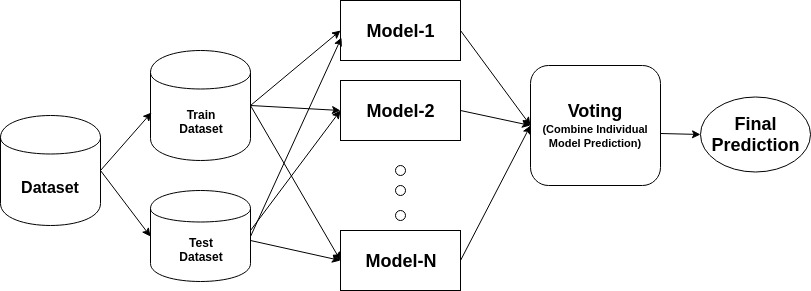
\includegraphics[width=0.6\linewidth]{img/Ensemble.png}
                \caption{Ensemble methods}
            \end{figure}
            \begin{enumerate}
                \item \textbf{Bagging} stands for bootstrap aggregation. It combines multiple learners in a way to reduce the variance of estimates. For example, random forest trains M Decision Tree, you can train M different trees on different random subsets of the 
                data and perform voting for final prediction. Bagging ensembles methods are Random Forest and Extra Trees;
                \item \textbf{Boosting algorithms} are a set of the low accurate classifier to create a highly accurate classifier. Low accuracy classifier (or weak classifier) offers the accuracy better than the flipping of a coin. Highly accurate classifier( or strong classifier) 
                offer error rate close to 0. Boosting algorithm can track the model who failed the accurate prediction. Boosting algorithms are less affected by the overfitting problem. The following three algorithms have gained massive popularity in data science competitions.
                    \begin{itemize}
                        \item AdaBoost (Adaptive Boosting)
                        \item Gradient Tree Boosting
                        \item XGBoost
                    \end{itemize}
                \item \textbf{Stacking (or stacked generalization)} is an ensemble learning technique that combines multiple base classification models predictions into a new data set. This new data are treated as the input data for another classifier. This classifier employed to 
                solve this problem. Stacking is often referred to as blending.
                    \begin{figure}[H]
                        \centering
                        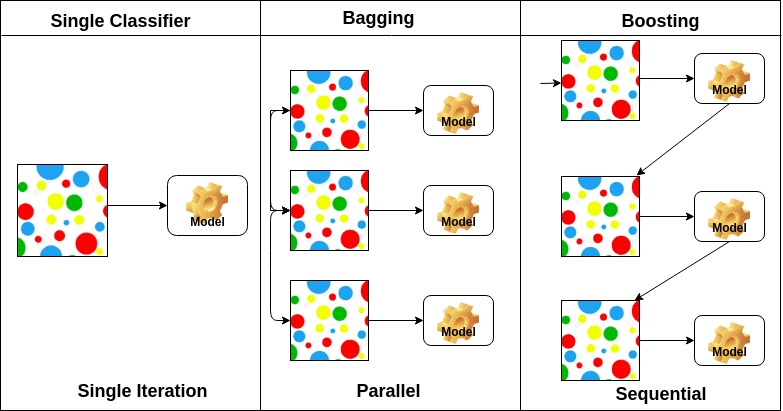
\includegraphics[width=0.6\linewidth]{img/stacking.png}
                        \caption{On the basis of the arrangement of base learners, ensemble methods can be divided into two groups: In parallel ensemble methods, base learners are generated in parallel for example. Random Forest. In sequential ensemble methods, base learners are generated sequentially for example AdaBoost.}
                    \end{figure}
            \end{enumerate}
            On the basis of the type of base learners, ensemble methods can be divided into two groups: homogenous ensemble method uses the same type of base learner in each iteration. heterogeneous ensemble method uses the different type of base learner in each iteration.
        \subsubsection{AdaBoost Classifier}
            Ada-boost or Adaptive Boosting is one of ensemble boosting classifier proposed by Yoav Freund and Robert Schapire in 1996. It combines multiple classifiers to increase the accuracy of classifiers. AdaBoost is an iterative ensemble method. 
            AdaBoost classifier builds a strong classifier by combining multiple poorly performing classifiers so that you will get high accuracy strong classifier. The basic concept behind Adaboost is to set the weights of classifiers and training the 
            data sample in each iteration such that it ensures the accurate predictions of unusual observations. Any machine learning algorithm can be used as base classifier if it accepts weights on the training set. Adaboost should meet two conditions:
            \begin{enumerate}
                \item The classifier should be trained interactively on various weighed training examples;
                \item In each iteration, it tries to provide an excellent fit for these examples by minimizing training error.
            \end{enumerate}
        \subsubsection{How Does AdaBoost Algorithm Work?}
            It works in the following steps:
            \begin{enumerate}
                \item Initially, Adaboost selects a training subset randomly;
                \item It iteratively trains the AdaBoost machine learning model by selecting the training set based on the accurate prediction of the last training;
                \item It assigns the higher weight to wrong classified observations so that in the next iteration these observations will get the high probability for classification;
                \item Also, It assigns the weight to the trained classifier in each iteration according to the accuracy of the classifier. The more accurate classifier will get high weight;
                \item This process iterate until the complete training data fits without any error or until reached to the specified maximum number of estimators;
                \item To classify, perform a "vote" across all of the learning algorithms you built.
            \end{enumerate}
            \begin{figure}[H]
                \centering
                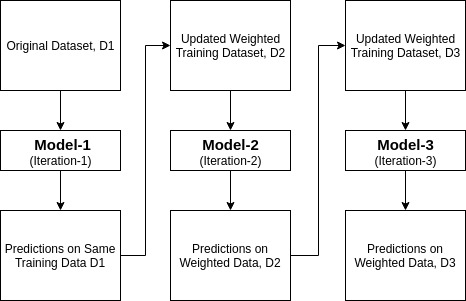
\includegraphics[width=0.6\linewidth]{img/Adaboost work.png}
                \caption{Adaboost model work}
            \end{figure}
            \begin{align}
                h_k = \left\{
                    \begin{array}{ll}
                        1 & \mbox{$p_k f_k(x) < p_k \theta_k$} \\
                        0 & \mbox{opposite}
                    \end{array}
                \right.
            \end{align}
            With: 
            \begin{itemize}
                \item $x$: Subwindow need to consider
                \item $\theta$: threshold
                \item $f_k$: Haar-like characteristic value
                \item $p_k$: Decision coefficient of detemining the dimension of the equation
            \end{itemize}
            Adaboost will combine weak classifiers into strong classifier as follows:
            \begin{align}
                H(x) = \Sigma(a_1 h_1(x) + a_2 h_2(x) +...+ a_n h_n(x))
            \end{align}
            With: $a_t >= 0$ is normalization coefficient for weak classifiers.
            \begin{figure}[H]
                \centering
                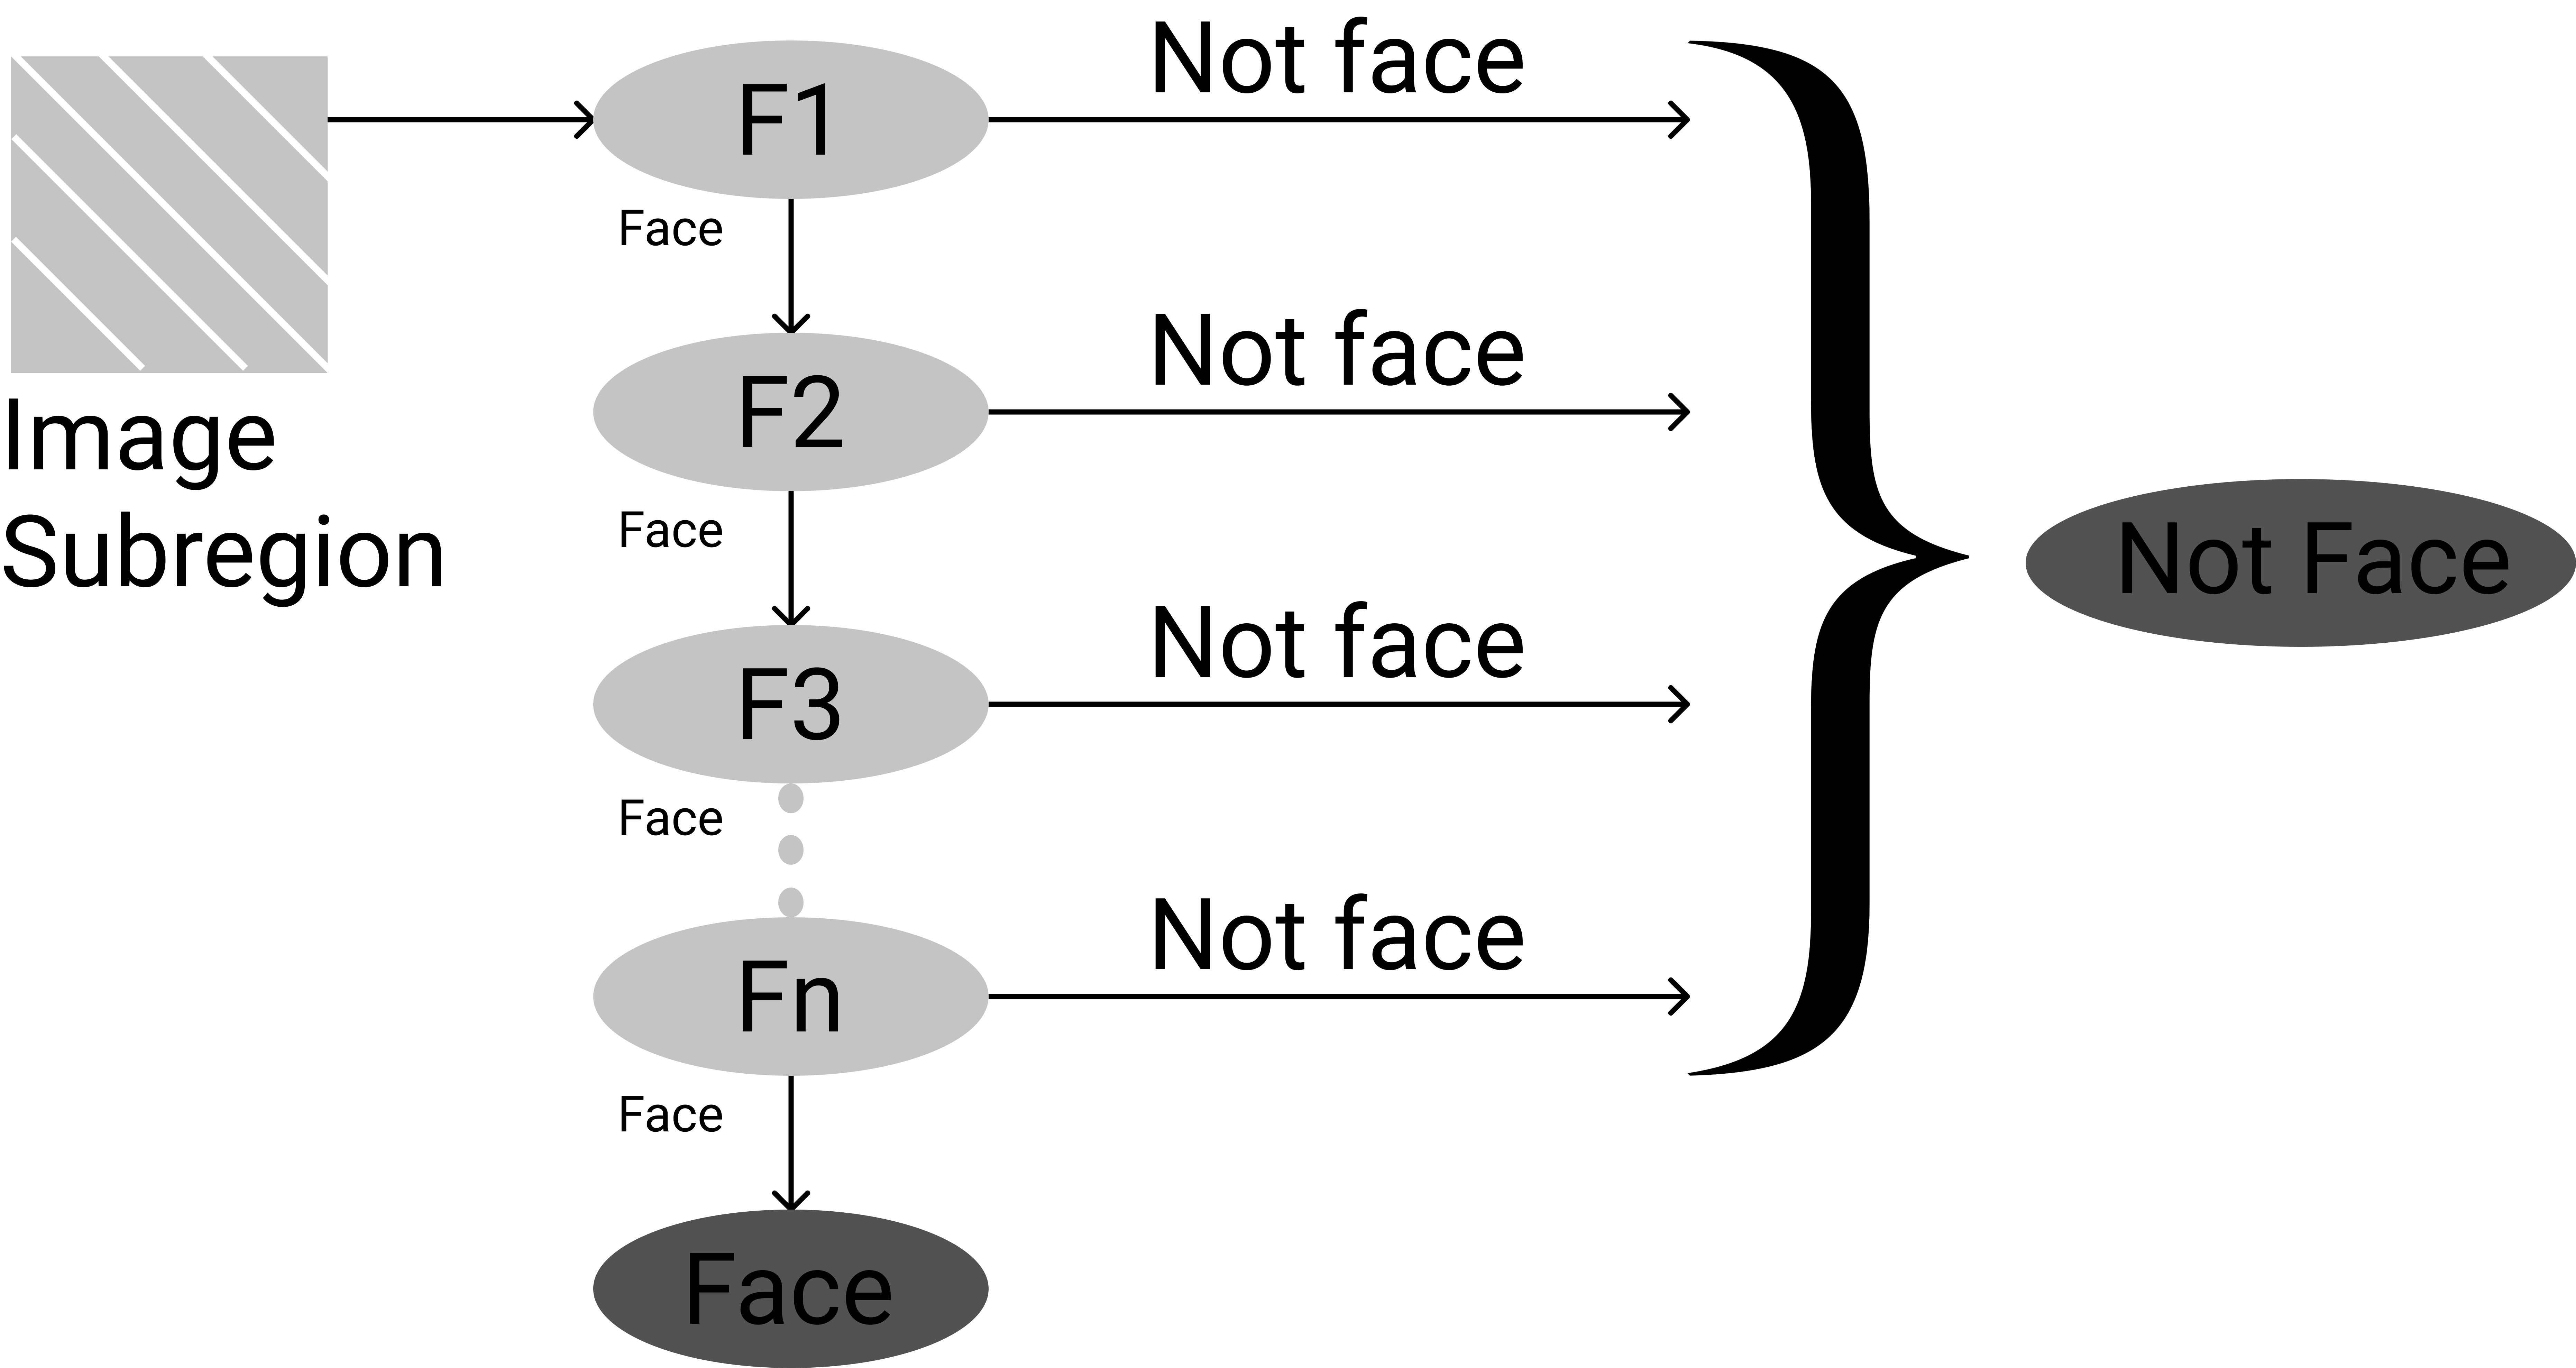
\includegraphics[width=0.6\linewidth]{img/Haar-Cascade.png}
                \caption{Haar Cascade Detection model}
            \end{figure}

\section{Euclidean Distance}

\section{OpenCV}

\section{Python Programming Language}

\section{Introduction about Dlib}

\section{Raspberry Pi 3B +}